% This is LLNCS.DEM the demonstration file of
% the LaTeX macro package from Springer-Verlag
% for Lecture Notes in Computer Science,
% version 2.4 for LaTeX2e as of 16. April 2010
%
\documentclass{llncs}
%
\usepackage{makeidx}  % allows for indexgeneration
\usepackage[pdftex]{graphicx}
%
\begin{document}
%
\mainmatter              % start of the contributions
%
\title{Deterministic Lazy Mutable OCL Collections}
%
\titlerunning{Deterministic OCL}  % abbreviated title (for running head)
%                                     also used for the TOC unless
%                                     \toctitle is used
%
\author{Edward D. Willink\inst{1}}
%
\authorrunning{Edward Willink} % abbreviated author list (for running head)
%
%%%% list of authors for the TOC (use if author list has to be modified)
\tocauthor{Edward Willink}
%
\institute{Willink Transformations Ltd, Reading, England,\\
\email{ed\_at\_willink.me.uk}}


\maketitle              % typeset the title of the contribution

\begin{abstract}
The Collection iterations and operations are perhaps the most important part of OCL.
It is therefore important for an OCL evaluation tool to provide efficient support for Collections. Unfortunately, some clauses of the OCL specification appear to inhibit efficient or deterministic support. We review the inhibitions and demonstrate a new deterministic and lazy implementation that avoids them.

\keywords{OCL, collection, deterministic, lazy, mutable}
\end{abstract}
%
\section{Introduction}
%
The OCL specification ~\cite{OCL-2.4} defines an executable specification language suitable for use with models. OCL's power comes from its ability to evaluate characteristics of multiple model elements using iterations and operations over collections.

The side-effect free functional characteristics of OCL should provide excellent opportunities for optimized evaluation, but sadly the optimization in typical OCL tools is poor. Collection evaluation is an area that should be particularly good, however it is very easy for the efficiency and/or memory usage to be outstandingly bad.

Deterministic execution is a desirable property of any language; very desirable if you are attempting to debug an obscure failure. Unfortunately today's OCL tools are not deterministic and so OCL-based Model-to-Model transformations tools also lack determinism. 

In Section~\ref{Problems}, we review the problems that the OCL specification appears to pose. In Section~\ref{Problems Revisited} we revisit these problems to identify over-enthusiastic or inappropriate reading of the OCL specification. Then in Section~\ref{Solutions} we introduce our new Collection implementation that solves the problems. The new solution is still work in progress and so in Section~\ref{Context and Status} we describe what remains to do to integrate it effectively. In Section~\ref{Related Work} we look at related work and conclude in Section~\ref{Conclusions}.
 
\section{The Problems}\label{Problems}

We briefly review some implementation challenges that the OCL specification provides.

\paragraph{Collection types:}

OCL defines an abstract $Collection$ type and four concrete derivations to support the four permutations of ordered/not-ordered, unique/not-unique content. These derived collections types are

\begin{itemize}
	\item $Bag$ - not-ordered, not-unique
	\item $OrderedSet$ - ordered, unique
	\item $Sequence$ - ordered, not-unique
	\item $Set$ - not-ordered, unique
\end{itemize}

Java implementations may use a custom class, \verb$LinkedHashSet$, \verb$ArrayList$ and \verb$HashSet$ to implement these four \verb$Collection$ types.

Problem: Four distinct collection types.

\paragraph{Immutability:}

OCL is a functional language free from side effects. It is therefore impossible to modify an OCL $Collection$. There are no operations such as \verb$Set::add(element)$ that modify the receiver. Rather there are operations such as \verb$Set::including(element)$ that return a new \verb$Set$ based on the receiver and including the additional \verb$element$. The obvious implementation of a cascade of operations such as \verb$a->including(b)->including(c)->including(d)$ creates a new intermediate collection between each operation.

Problem: Immutability implies inefficient collection churning.

\paragraph{Eagerness:}

OCL operations are defined as a computation of an output from some inputs. A cascade of operations such as \verb$a->including(b)->excludes(c)$ is therefore evaluated in three steps as get-\verb$a$, create \verb$a+b$, test \verb$a+b$ for \verb$c$ content. There is no mechanism for early discovery of a \verb$c$ to bypass redundant computations.

Problem: Specification implies eager evaluation.

\paragraph{Invalidity:}

A malfunctioning OCL evaluation does not throw an exception, rather it returns the \verb$invalid$ value, which will normally be propagated through invoking computations back to the caller. However OCL has a strict Boolean algebra that allows the \verb$invalid$ value to be `caught' when, for instance, ANDed with the \verb$false$ value. The presence of the \verb$invalid$ value in a collection is prohibited, or rather the whole collection that `contains' the \verb$invalid$ value is replaced by the \verb$invalid$ value. The result of a collection evaluation cannot therefore be determined until every element is present and checked for validity.

Problem: Invalidity implies full evaluation.

\paragraph{Determinism:}

Each collection type has distinct useful capabilities and so conversions between collection types are specified to facilitate their use. However, when the \verb$asOrderedSet()$ and \verb$asSequence()$ operations are applied to not-ordered collections, the operations must create an ordering without any clue as to what a sensible ordering criterion might be. This is obviously impossible and so typical Java implementations use the indeterminate order provided by a Java iteration over an underlying Java \verb$Set$.

Problem: \verb$asOrderedSet()$ and \verb$asSequence()$ imply indeterminacy.

\paragraph{OCL equality:}

OCL is a specification language and when dealing with numbers, OCL uses unbounded numbers. Consequently the following OCL expressions are true:
\begin{verbatim}
1 = 1.0  Set{1,1.0}->size() = 1  Set{Set{1},Set{1.0}}->size() = 1
\end{verbatim}
When using Java to implement OCL, the numeric equality is satisfied by the primitive types \verb$int$ and \verb$double$ but not by the object types \verb$Integer$ and \verb$Double$. Since Java sets use object equality to establish uniqueness, a naive implementation that assumes that OCL and Java equality are the same may malfunction.

Problem: OCL and Java equality semantics are different.

%OCL's use of unbounded numbers is also an efficiency challenge since using Java's \verb$BigInteger$ throughout would be undesirable. However once a Facade is introduced to solve the OCL equality problem, the Facade can also hide a variety of polymorphic representations.

\section{The Problems Revisited}\label{Problems Revisited}

The foregoing problems lead to poor and even inaccurate OCL implementations. We will therefore examine them in more detail to distinguish myth and truth before we introduce our new solution.

%\subsection{Primitives}\label{Primitives}

%OCL exploits the UML Boolean, Integer and Real primitives that have obvious Java counterparts in boolean, int and double. However OCL specifies unlimited precision for which int is unsuitable and so BigInteger (and BigDecimal) are more appropriate. But the Java equality semantics for objects and primitives is different and so direct use of Java objects rather than primitives gives the wrong result for the OCL expression "1 = 1.0". It is undesirable to use BigInteger for all integer values since for most applications all integer could be much more efficiently supported by a simple Java Integer.

%A practical implementation may resolve these conflicts by introducing IntegerValue and RealValue interfaces with a variety of precision implementations such as IntIntegerValue, LongIntegerValue and BigIntegerValue. The IntIntegerValue can wrap an int in exactly the same way as the normal Java Integer class and so avoid any size overheads for the dominant use case. However equality and addition can be reimplemented to provide the OCL equality semantics and growth to a higher precision class rather than an ill-disciplined wraparound.

%\subsubsection{UnlimitedNatural}

%UML and OCL have an additional UnlimitedNatural primitive to support the upper bound of a UML multiplicity. It has no negative values and so appears to be a subtype of Integer, however it also has an unlimited "*" value which converts to Integer as an invalid value. UnlimitedNatural is therefore irregular and so it is better to treat it as a distinct kind of type such as an EnumerationLiteral with explicit conversions rather than as a regular part of the IntegerValue, RealValue number system with implicit conversions.

%\subsection{Tuples}

%A Tuple provide a set of named elements. This may be easily implemented using a Java Map from name to value. A more space-efficient representation can use just a Java array of values ordered by the alphabetical ordering of their names. Generated code may even use the indexes rather than the names to accelerate access.

\subsection{Immutability}

While OCL may provide no operations to modify Collections, it does not prohibit modification by underlying tooling, provided the modification does not affect the OCL execution.

An evaluation of \verb$a->including(b)->including(c)$ may therefore re-use the intermediate collection created by \verb$a->including(b)$ and modify it to create the final result. This is safe since the intermediate result cannot be accessed in any other way than by the subsequent \verb$->including(c)$. If there are no other accesses to \verb$a$, it is permissible to
modify \verb$a$ twice and avoid all intermediates.

\subsection{Eagerness}

While the specification may imply that evaluations should be performed eagerly, this is just the way specifications are written to ease understanding. An implementation is permitted to do something different so long as the difference is not observable. Lazy evaluation is a tactic that has been used with many languages. OCL has a strong functional discipline and so laziness has much to offer in an OCL evaluator. Unfortunately OCL development teams have been slow to exploit this optimization.

\subsection{Invalidity}

The OCL specification is far from perfect. In OCL 2.0, there were the three overlapping concepts of $null$, $undefined$ and $invalid$. OCL 2.2 clarified the concepts by eliminating $undefined$ and so distinguished $null$ and $invalid$, but $invalid$ is still inadequate to represent real execution phenomenon.

There is currently no distinction between program failures such as
\begin{itemize}
	\item divide by zero
	\item $Sequence$/$OrderedSet$ index out of range
	\item $null$ navigation
\end{itemize}

and machine failures such as
\begin{itemize}
	\item stack overflow
	\item network failure
\end{itemize}

Since machine failures are not mentioned by the specification, it would seem that they must be \verb$invalid$, but few programs are expected to return a useful result in the event of a machine failure. Consequently the treatment of machine failures as \verb$invalid$ for the purposes of 4-valued (\verb$true$,\verb$false$,\verb$null$,\verb$invalid$) strict logic evaluation seems misguided. Rather a further fifth \verb$failure$ value for machine failure should be non-strict so that machine failures are not catchable by logic guards. The fourth strict \verb$invalid$ value should apply only to program failures.

Program failures are amenable to program analysis that can prove that no program failure will occur. When analysis is insufficiently powerful, the programmer can add a redundant guard to handle e.g. an `impossible' divide-by-zero. With 5-valued logic we can prove that the partial result of a collection evaluation will remain valid if fully evaluated and so avoid the redundant full calculation when the partial calculation is sufficient.

Proving that null navigations do not occur is harder but an analysis of null safety is necessary anyway to avoid run-time surprises~\cite{Safe OCL}.

Once machine failures are irrelevant and the absence of program failures has been proved, a partial collection result may be sufficient; the redundant evaluations can be omitted.

\subsection{Determinism}

Determinism is a very desirable characteristic of any program evaluation, particularly a specification program. Is OCL really non-deterministic?
 
\verb$Collection::asSequence()$ is defined as returning elements in a collection kind-specific order.

The \verb$Set::asSequence()$ override refines the order to $unknown$, which is not the same as $indeterminate$. 

The foregoing appears in the normative part of the specification. Only the non-normative annex mentions a lack of determinism.

It is therefore unclear from the specification text whether an OCL implementation may be non-deterministic. A clarified OCL specification could reasonably take either alternative.

In practice, typical OCL implementations use a Java \verb$Set$ to realize OCL $Set$ functionality. The iteration order over a Java \verb$Set$ depends on hash codes, which depend on memory addresses, which depend on the unpredictable timing of garbage collection activities. It is therefore not possible for typical OCL implementations to be deterministic. 

It would appear that implementation pragmatics are driving the specification or at least the user perception of the specification. But indeterminacy is so bad that it would be good to find a way to make OCL deterministic.

\subsection{Four Collection types}

The four permutations of unique and ordered provide four collection behaviors and four specification types, but do we really need four implementation types? With four types we may have the wrong one and so we need conversions. UML~\cite{UML-2.5} has no collection types at all. What if an implementation realized all four behaviors with just one implementation type? One benefit is obvious; no redundant conversions.

\section{New Collection Solution}\label{Solutions}

Our new solution has only one $Collection$ implementation type that exhibits all four $Collection$ behaviors, but only one at a time. To avoid confusion between our new $Collection$ implementation and the OCL abstract $Collection$ or the Java \verb$Collection$ classes, we will use \verb$NewCollection$ in this paper\footnote{The Eclipse OCL class name is currently LazyIterable}.

\subsection{Deterministic Collection Representation}

A \verb$NewCollection<T>$ instance uses two Java collection instances internally.

\begin{itemize}
	\item \verb$ArrayList<T>$ of ordered elements.
	\item \verb$HashMap<T,Integer>$ of unique elements and their repeat counts.
\end{itemize}

For a $Sequence$, the \verb$ArrayList$ serializes the required elements. The \verb$HashMap$ is unused and may be \verb$null$.

For a $Set$, the keys of the \verb$HashMap$ provide the unique elements each mapped to a unit \verb$Integer$ repeat count. The \verb$ArrayList$ serializes the unique elements in a deterministic order.

For an $OrderedSet$, the keys of the \verb$HashMap$ provide the unique elements each mapped to a unit \verb$Integer$ repeat count. The \verb$ArrayList$ serializes the unique elements in the required order.

For a $Bag$, the keys of the \verb$HashMap$ provide the unique elements each mapped to a repeat count of that element. The \verb$ArrayList$ serializes the unique elements in a deterministic order.

The Java implementation of a \verb$HashSet$ uses a \verb$HashMap$ and so using a \verb$HashMap$ for $Set$ and $OrderedSet$ incurs no additional costs. On a 64 bit machine, each \verb$HashMap$ element incurs a 44 byte cost per \verb$Node$ and typically two 8 byte costs for pointers. Using an \verb$ArrayList$ as well as a \verb$HashMap$ increases the cost per entry from 60 to 68 bytes; a 13\% overhead for non-$Sequence$s.

Use of an \verb$ArrayList$ to sequence the unique elements for all forms of $Collection$ allows an efficient deterministic iterator to be provided for all kinds of $Collection$.

For a $Bag$, there is a choice as to whether an element iteration is over all elements, repeating repeated elements, or just the unique elements. The \verb$NewCollection$ therefore provides a regular \verb$iterator()$ over each element, and a \verb$bagIterator()$ that skips repeats but allows the repeat count to be accessed by the iterator. $Bag$-aware implementations of $Collection$ operations can therefore offer a useful speed-up.

Since a $Set$ now has a deterministic order, there is no implementation difference between a $Set$ and an $OrderedSet$.

The deterministic order maintained by the \verb$ArrayList$ is based on insertion order. New elements are therefore added at the end or not at all, which avoids significant costs for \verb$ArrayList$ maintenance.

The \verb$NewCollection$ supports all $Collection$ behaviors, but only one at a time. Non-destructive conversion between behaviors can be performed as no-operations. A $Set$ converts to a $Sequence$ by continuing to use the \verb$ArrayList$ and ignoring the \verb$HashMap$. However the conversion from a $Sequence$ to a $Bag$ or $Set$ requires the \verb$HashMap$ to be created and non-unique content of the \verb$ArrayList$ to be pruned; a new \verb$NewCollection$ is therefore created to avoid modifying the original \verb$NewCollection$.

The \verb$NewCollection$ does not inherit inappropriate Java behavior. The problems with inconsistent OCL/Java equality semantics can therefore be resolved as \verb$NewCollection$ delegates to the internal \verb$HashMap$.

\subsection{Deterministic Collection Cost}

Fig~\ref{fig:SetCreatePerformance} contrasts the performance of creating instances of the `old' Eclipse OCL $Set$ with the `new' NewCollection $Set$. log-log axes show the time to create a $Set$ from a $Sequence$ of distinct integers. Overall the `new' design is about 2 times slower corresponding to the use of two rather than one underlying Java collection.

\begin{figure}
	\begin{center}
		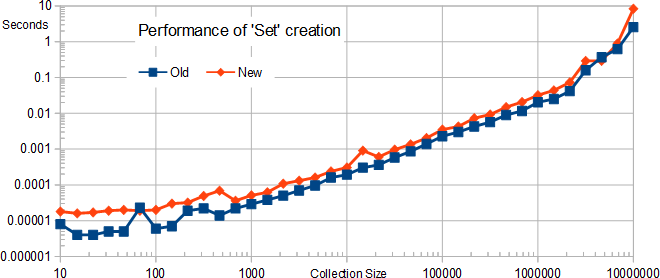
\includegraphics[width=4.5in]{SetCreatePerformance.png}
	\end{center}
	\caption{`Set' Creation Performance}
	\label{fig:SetCreatePerformance}
\end{figure}

A corresponding contrast of iteration speed is shown in Fig~\ref{fig:SetIteratePerformance}. The `new' design is now about three times faster since the iteration just traverses adjacent entries in the deterministic \verb$ArrayList$ rather than the sparse tree hierarchy of non-deterministic \verb$HashMap$ nodes.

\begin{figure}
	\begin{center}
		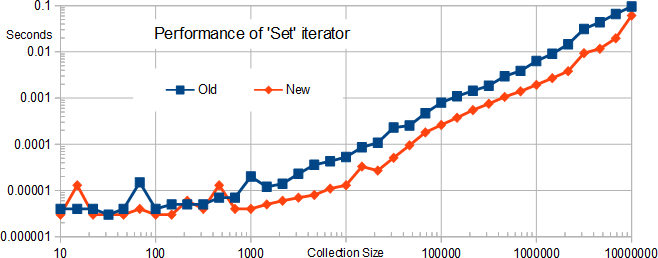
\includegraphics[width=4.5in]{SetIteratePerformance.png}
	\end{center}
	\caption{`Set' Iteration Performance}
	\label{fig:SetIteratePerformance}
\end{figure}

Iteration is faster than creation and so it depends how often the $Set$ is used as to whether `new' or `old' is faster overall. More than three uses and the `new' design is faster as well as deterministic. Even when used only once the speed penalty is less than a factor of two. Determinism is therefore practical and incurs acceptable size and speed costs. 

\subsection{Lazy Usage}

The `eager' exposition of \verb$NewCollection$'s \verb$ArrayList$ solves the problem of indeterminacy. The lazy use of a \verb$HashMap$ as well as the \verb$ArrayList$ supports conversions and non-$Sequence$ collections.

The \verb$NewCollection$ may also be be used for lazy evaluation by providing careful support for Java's \verb$Iterator$ and \verb$Iterable$ interfaces.

When a \verb$NewCollection$ has a single consumer, its \verb$Iterator$ may be used directly by invoking \verb$iterator()$ to acquire an output iterator that delegates directly to the input.

When a \verb$NewCollection$ has multiple consumers, it must be used as an \verb$Iterable$ to provide a distinct \verb$Iterator$ for each consumer. \verb$iterable()$ is invoked to activate the caching that then uses an internal iterator to iterate over the input at most once.

Considering: \verb$a->including(b)->including(c)$

An eager implementation of \verb$Collection::including$ might be implemented by the \verb$IncludingOperation.evaluate$ method as shown in Fig~\ref{fig:EagerExample}. 

\begin{figure}
	\begin{center}
		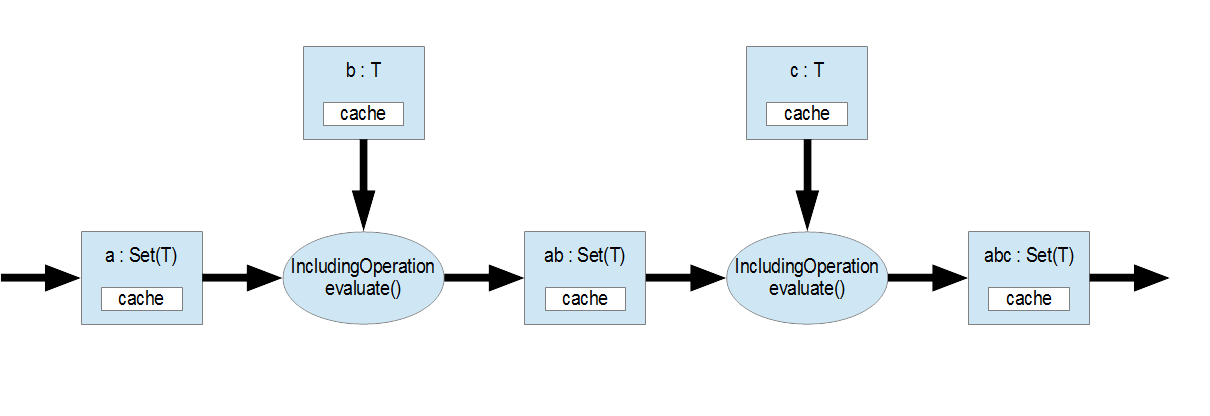
\includegraphics[width=4.5in]{EagerExample.png}
	\end{center}
	\caption{Example Eager Evaluation Data Flow}
	\label{fig:EagerExample}
\end{figure}

The stateless \verb$IncludingOperation::evaluate()$ eagerly accesses the \verb$a$ and \verb$b$ values cached by their Variable objects and creates the intermediate \verb$ab$. A second \verb$IncludingOperation::evaluate()$ similarly produces the result \verb$abc$. Three collection caches are fully populated for each of \verb$a$, \verb$ab$ and \verb$abc$.

The lazy implementation shown in Fig~\ref{fig:LazyExample} uses an \verb$IncludingIterator$ object that has a \verb$current$ iteration context. The iterator iterates to produce the required output, one element at a time by fetching the inputs one element at a time and interleaving the additional value at the correct position. No computation is performed until an attempt is made to access the \verb$abc$ result. Since the result cache is missing, the \verb$abc$ access invokes \verb$IncludingIteration::next()$ to provide each element of \verb$abc$ that is required. \verb$IncludingIterator::next()$ provides its result from \verb$c$ or by invoking \verb$next()$ on \verb$ab$, which in turn acquires its values from \verb$a$ or \verb$b$. No input, intermediate or output collection caches are required; \verb$a$ can read its source one element at a time, \verb$ab$ relays its values one at a time, and the \verb$abc$ output may be accessed one element at time. This is a major size improvement, three uncached \verb$NewCollections$ that relay one element at a time, rather than three fully-cached \verb$NewCollection$s.

\begin{figure}
	\begin{center}
		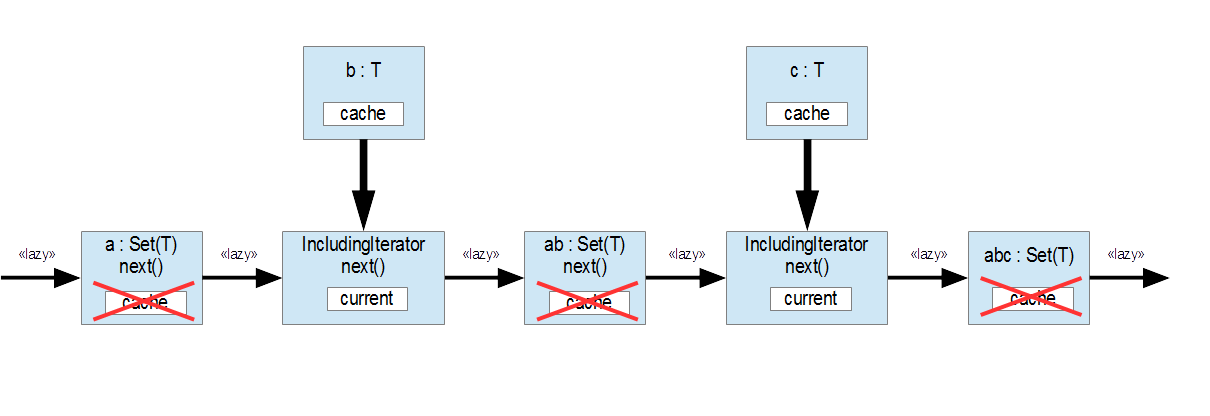
\includegraphics[width=4.5in]{LazyExample.png}
	\end{center}
	\caption{Example Lazy Evaluation Data Flow}
	\label{fig:LazyExample}
\end{figure}

If \verb$a$ or \verb$c$ has multiple consumers, as shown in Fig~\ref{fig:LazyCachedExample}, the undesirable repetition of the lazy including computations is avoided by activating caches where the multi-use occurs. This is slightly awkward to implement since the first consumer must invoke \verb$NewCollection.iterable()$ to activate the cache before any consumer invokes \verb$NewCollection.iterator()$ to make use of the collection content. As part of a general purpose library used by manual programmers this programming discipline could cause many inefficiencies. However as part of an OCL tool, an OCL expression is easily analyzed to determine whether a collection variable is subject to multiple access. If analysis fails, \verb$iterable()$ can be invoked just in case.

\begin{figure}
	\begin{center}
		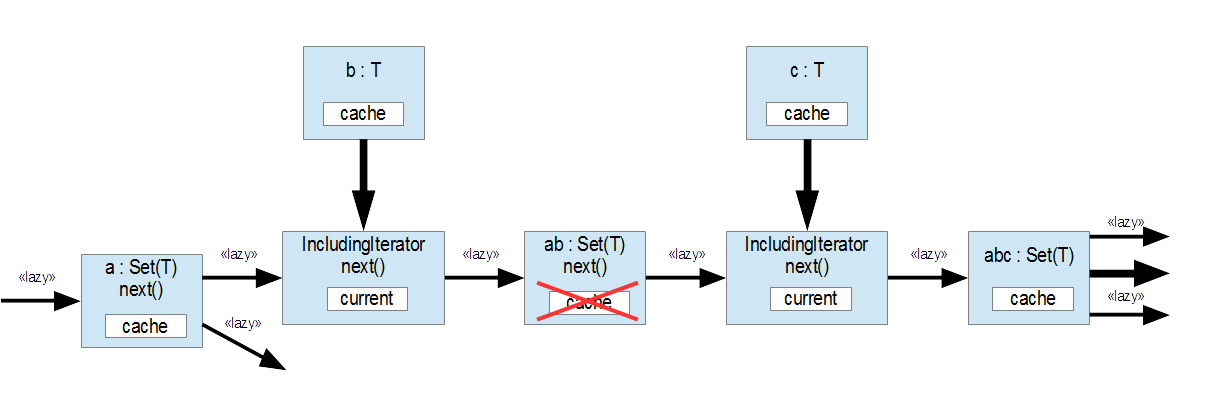
\includegraphics[width=4.5in]{LazyCachedExample.png}
	\end{center}
	\caption{Example Lazy Cached Evaluation Data Flow}
	\label{fig:LazyCachedExample}
\end{figure}

Eager, lazy and cached evaluations share the same structure of operation and variable interconnections. The correct behavior is configured by an analysis of the OCL expression to identify whether the collection subject to single access permitting a transparent behavior or multiple access requiring a cached behavior in which the source iteration is lazily cached for multiple use by the multiple accesses. Unfortunately, collection operations, such as \verb$Collection::size()$, are unable to return a result until the source has been fully traversed  lazy access and so an eager evaluation is sometimes unavoidable.

\subsection{Lazy Cost}

In Fig~\ref{fig:DoubleIncludingPerformance} we contrast the performance of eager and lazy OCL evaluation of the inclusion of two values into a $Sequence$ of $Integer$s. 

\begin{figure}
	\begin{center}
		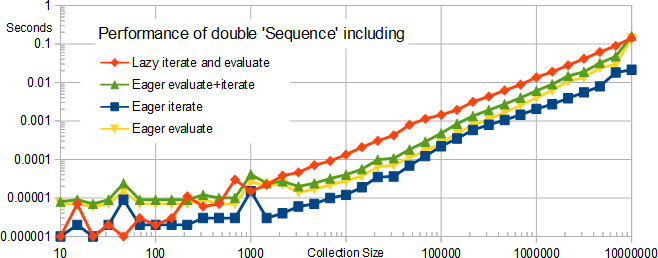
\includegraphics[width=4.5in]{DoubleIncludingPerformance.png}
	\end{center}
	\caption{Double Including `Sequence' Performance}
	\label{fig:DoubleIncludingPerformance}
\end{figure}

For more than 1000 elements, the top curve shows the lazy approach scaling proportionately. The next curve shows the aggregate performance of eager evaluation also scaling proportionately until garbage collection affects results at 10,000,000 elements. The bottom two curves show the contributions to the aggregate from the eager evaluation, and the final result traversal.

For small $Sequence$s with fewer than 1000 elements, the higher constant costs of the eager approach dominate and the lazy approach is perhaps five times faster.

For larger $Sequence$s, the lazy approach is about two times slower since an outer element loop traverses iterations for each partial computation whereas the eager approach has tighter inner loops for each partial computation.

For the largest 10,000,000 element result, garbage collection has started to affect the eager evaluation with its three full size  collection values for input, intermediate and output. In contrast, the lazy approach only uses a few hundred bytes regardless of model size and so is much less affected by huge models.

The lazy approach is clearly superior with respect to memory consumption, and also faster for up to about 1000 elements. For larger sequences, lazy evaluation may be two times slower. Since lazy evaluation offers the opportunity to skip redundant computations, we may conclude that in the absence of application-specific profiling measurements, lazy evaluation should be used.

%\subsection{Collections}

%Collections (and their operations/iterations) are perhaps the most important part of OCL and so an efficient representation is important. The OCL Collection has an obvious counterpart in a Java Collection. The OCL Sequence and Set have similarly obvious counterparts in Java's ArrayList and HashSet. OCL's OrderedSet is similar to a Java LinkedHashSet, although LinkedHashSet ignores the ordering for the purposes of equality testing. OCL's Bag has no counterpart and so must be hand-coded.

%Java's set operations make use of hashCode() and equals() methods and so we find that the problem with "1 = 1.0" reappears as "Set{1, 1.0}->size()". Avoiding evaluation of "1 = 1.0" is possible. Avoiding inconsistent Set content treatment is much harder when Java Sets are used as is.

%It is often necessary to convert an OCL collection such as a Bag returned by a collect to another collection such as a Set to exploit its uniqueness properties. If a distinct Java collection is used for each OCL collection, each conversion requires the creation of a new Java collection.

%Creation of new collection conversions is just the tip of the iceberg for inefficient collection evaluation. A manually coded asSet() such as

%$Sequence{1,2,3,2,1}->iterate(i; acc:Set(Integer) | acc->including(i))$

%may churn four intermediate accumulations before creating the useful collection result. A notionally linear problem incurs quadratic execution costs. For large
%models and non-trivial collection expressions, it is very easy for eager OCL evaluation that respects the immutability of OCL collections to have very disappointing performance.

%\section{The Solutions2}

%We have identified that the eager evaluation of collection operations can be expensive. For some calculations it can be very expensive, for instance

%$aCollection->isEmpty()$

%does not require every element of $aCollection$ to be calculated; it is sufficient to know that there is, or is not, an element. If $aCollection$ was computed lazily then considerable eager computation could be saved.


%\subsubsection{Lazy Collection evaluations}

%The unified collection representation eliminates conversion costs, but this is unlikely to exceed 25\% of the overall collection evaluation costs. For really significant improvements we need to eliminate redundant calculations and redundant intermediates. This can be achieved by lazy evaluation.

%inv ExtendedTypedModelIsExtended:
%_extends <> null implies
%_extends.modelParameter->forAll(etm |
%self.modelParameter->select(name = etm.name).usedPackage->includesAll(etm.usedPackage)
%)

\subsection{Mutable Collections}

As suggested above, lazy evaluation is not always better. The simple example in Fig~\ref{fig:LazyExample} replaced three fully-cached by three uncached \verb$NewCollection$s but also introduced two intervening \verb$IncludingIterator$ objects. Invocation of \verb$next()$ to return an output object traverses the lazy sources incurring four nested invocations of \verb$next()$. For an iteration such as

\begin{verbatim}
aCollection->iterate(e; acc : Set(String) |
    acc->including(e.name))
\end{verbatim}

the overall iterate of an $N$-element \verb$aCollection$ evaluates using a chain of $N$ interleaved \verb$NewCollection$ and \verb$IncludingIterator$ objects. The overall evaluation incurs a quadratic $2*N*N$ cost in \verb$next()$ calls.

Of course the traditional approach of creating a new Collection for each invocation of \verb$including$ also incurs a quadratic cost through creating and copying $N$ collections of approximately $N$-element size.

In order to achieve a more reasonable cost we can use a non-OCL mutable operation behind the scenes:

\begin{verbatim}
aCollection->iterate(e; acc : Set(String) |
    acc->mutableIncluding(e.name))
\end{verbatim}

This exploits the invisibility of the intermediate values of \verb$acc$. The evaluation should therefore analyze the OCL expression to detect that the single use of \verb$acc$ allows the immutable \verb$including()$ operation to be evaluated safely and more efficiently using the internal \verb$mutableIncluding()$ operation. 

In Fig~\ref{fig:AccumulationPerformance} we contrast the performance of the accumulation that computes 

\verb$S->iterate(i; acc : C(Integer) = C{} | acc->including(i))$

using \verb$Set$ or \verb$Sequence$ as the \verb$C$ collection type and \verb$C{1..N}$ as the \verb$S$ source value for an \verb$N$ collection size.

The new approach uses mutable evaluation to re-use \verb$acc$ and so avoid churning.
The old approach uses the one new $Set$ churn per \verb$Set::including$ execution as currently practiced by Eclipse OCL~\cite{Eclipse-OCL} and USE~\cite{USE} (Dresden OCL~\cite{Dresden-OCL} creates two $Set$s). The new approach scales linearly and so is clearly superior to the traditional quadratic cost. The new approach has a two-fold cost for using $Set$s rather $Sequence$s; much less than when churning occurs.

\begin{figure}
	\begin{center}
		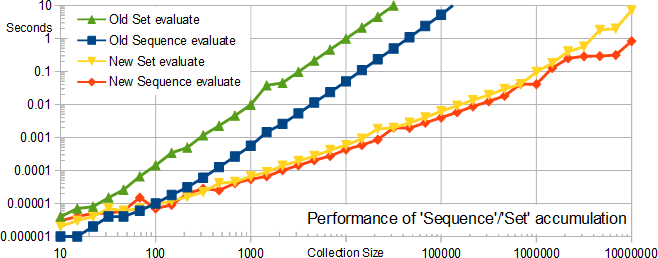
\includegraphics[width=4.5in]{AccumulationPerformance.png}
	\end{center}
	\caption{`Sequence' and `Set' Accumulation Performance}
	\label{fig:AccumulationPerformance}
\end{figure}

%The problem with eager intermediate collections can be mitigated by re-using the intermediates. In the example above the incoming accumulator is redundant at the end of the iteration and so could be re-used for the output accumulator. If the implementation recognizes this redundancy the "including" that creates a new collection based on the old can instead mutate the old. The particular case of an iteration accumulator is rather easy to recognize. 

Note that this optimization relies on a `compile-time' OCL expression analysis that replaces \verb$including$ by \verb$mutableIncluding$.

%More general redundancy and rewriting is much harder and probably less effective than the lazy evaluation we will now describe.


\subsection{Lazy limitations}

Some operations such as \verb$aCollection->size()$ cannot be executed lazily since the size cannot be known without the whole collection. But in a suitable context such as \verb$aCollection->size() > 3$, it is obvious that the full collection is not necessary after all. Even for \verb$aCollection->size()$, \verb$aCollection$ does not need to be fully evaluated since we are only interested in the number of elements. If the computation of \verb$aCollection$ can be aware that only its size is required, a more efficient existence rather than value of each element might be computed.
 
\subsection{Operation caches}

As well as using `lazy' evaluation to defer computation in the hope that it may prove redundant, performance may be improved by caching what has already been computed in the hope that it can be re-used.

As a side-effect free language, OCL is very well suited to caching the results of iteration or operation calls. However for simple arithmetic, short strings and small collections, the cost of caching and re-use may easily exceed the cost of re-computation. For larger collections, the cache size may be unattractive and the probability of re-use too low. Such dubious benefits perhaps explain the reticence of implementations to provide result caching.

Model to model transformations depend on re-use of created output elements and so the Eclipse QVTd tooling~\cite{Eclipse-QVTd} pragmatically provides caches for Functions and Mappings but not Operations or Iterations.

Empirical observation suggest that for object operations and derived properties, the re-use benefits and statistics are much more favorable and so such caching should be part of an OCL evaluator. We will shortly see another example where operation caching can be helpful.

\subsection{Smart select}

The $select$ iteration applies a Boolean predicate to filter a source collection.

\verb$sourceCollection->select(booleanPredicate)$

In practice there are two common idioms associated with $select$.

\subsubsection{Conformance selection:}

It is very common to use

\begin{verbatim}
S->select(oclIsKindOf(MyType)).oclAsType(MyType)
\end{verbatim}

This selects those elements of \verb$S$ that conform to \verb$MyType$. This clumsy test and cast idiom was recognized in OCL 2.4 and a \verb$selectByKind()$ operation added to improve readability.

In practice each source collection is partitioned into a very small number of types that can be identified by compile-time analysis of the OCL expressions. A naive implementation may recategorize the type of each element in each invocation. A more efficient implementation should re-use the type categorization to partition into all types of interest on the first invocation and cache the partitions for re-use by subsequent invocations for any of the types of interest. This should of course only be performed after Common Sub Expression or Loop Hoisting has eliminated redundant invocations, and only if there is more than one residual invocation.

\subsubsection{Content selection:}

It is also common to use

\begin{verbatim}
S->select(element | element.name = wantedName)
\end{verbatim}

This locates a matching content of \verb$S$by choosing the appropriately named elements. This idiom treats the \verb$S$ as a \verb$Map$ with a \verb$name$ key, but whereas a \verb$Map$ returns the value in constant time, naive implementation of $select$ incurs linear search cost.

For a single matching lookup, building the \verb$Map$ incurs a linear cost and so there is no benefit in an optimization. However in a larger application it is likely that the name lookup may occur a few  times for the same name and many times for different names. Providing an underlying \verb$Map$ may be very beneficial, converting a quadratic performance to linear.

%An iteration such as \verb$aCollection->select(element | element.name = wantedName)$ is the OCL idiom for locating typically just one element that matches a criterion, such as a name. The naive implementation just iterates over the collection and returns all matches. This is unavoidable for a simple query that performs just a single lookup, but in a larger application the lookup may be repeated many times to locate the same or other names. The repeated lookups will probably result in a quadratic performance. The quadratic cost can be avoided by building an index once and then looking up the wanted value in the index rather than searching for it. Building the index should be beneficial whenever more than one lookup is performed. The index can be managed by the source collection with potentially a distinct index for each \verb$aCollection->select(element | f(element) = ...)$ consumption.

We will contrast the performance, with and without a \verb$Map$, of the accumulation that computes 

\begin{verbatim}
let S = Sequence{1..N} in
let t = S->collect(i|Tuple{x=i}) in
S->collect(i | t->select(x = i))
\end{verbatim}

The first two $let$ lines build the table all of whose entries are looked up by the final line.

The top line of Fig~\ref{fig:SelectionPerformance} shows the traditional naive full search for each lookup. The lower lines show the time to build the cache, the time to perform all lookups and their sum. The \verb$Map$ is clearly helpful for anything more than one lookup. As expected, it scales linearly rather than quadratically.

\begin{figure}
	\begin{center}
		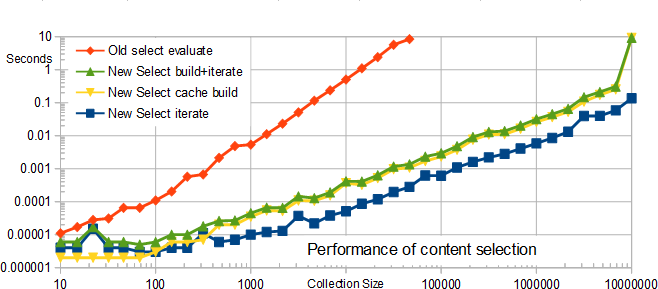
\includegraphics[width=4.5in]{SelectionPerformance.png}
	\end{center}
	\caption{`select' Performance}
	\label{fig:SelectionPerformance}
\end{figure}
  
\section{Context and Status}\label{Context and Status}

The OCL tooling must perform OCL expression analyses to use the foregoing \verb$NewCollection$ capabilities effectively
\begin{itemize}
	\item Identify mutable collections - use alternative mutable operation
	\item Identify single/multiple use collections - configure shared laziness
	\item Identify content selects - configure lookup tables
\end{itemize}

However since OCL by itself is useless, OCL tooling cannot know whether or how to optimize. It is only when OCL is embedded in a larger application that provides the models and the related OCL expressions that OCL becomes useful.

For the simplest OCL application in which an interactive OCL expression is evaluated with respect to a model, the costs of the model and expression analyses may easily outweigh the benefits. No optimization may well give the snappiest interactive response.

For a more complex OCL application such as the OCL definition of model constraints, operations and properties supported by OCLinEcore, Eclipse OCL provides a code generator~\cite{OCL-CG} that embeds the Java for the OCL within the Java for the Ecore model.

The code generator performs a variety of compile-time analyses and syntheses:
\begin{itemize}
	\item Common SubExpression / Loop hoisting
	\item Constant Folding
	\item Inlining
	\item Dispatch tables
\end{itemize}

The code generator also prepares tables and structures that cannot be fully analyzed until
the actual run-time models are available:
\begin{itemize}
	\item Run-Time Type Information (e.g. oclIsKindOf support)
	\item Run-Time Navigability Information (unnavigable opposites)
	\item Run-Time Instances Information (allInstances)
\end{itemize}
Adding a few additional activities is structurally easy, and only a minor compile-time degradation. The results presented earlier use a manual emulation of what the automated analysis and synthesis should achieve~\footnote{Unifying the four concrete Collection types by a single replacement presents some compatibility challenges that may require Ec;lipse OCL to make a major version number change. The code for lazy evaluations is therefore only available on the ewillink/509670 branch in the Eclipse OCL GIT repository}.

For OCL-based applications such as QVTc or QVTr~\cite{QVT-1.3}, the Eclipse OCL code generator has been extended and appears to provide a twenty-fold speed-up compared to less optimized interpreted execution~\cite{Willink-EXE2016}. A smaller speed-up is to be expected for intensive $Collection$ computations where most of the execution occurs in shared run-time support such as \verb$Set::intersection()$.

%\subsection{Compile-time / Load-time analyses}

%The compile-time analysis has 100\% of the OCL available for global analysis. This enables run-time computations to be identified in advance and custom run-time structures to be synthesized.
 
%\subsubsection{Unnavigable opposites}

%Naive execution of an unnavigable opposite is very expensive since it requires a substantial search of the model to find the target object that points at the particular source. If all such navigations are pre-identified, a single traversal of the model can cache all opposites reducing the subsequent cost to a cache access.

%In practice very few unnavigable navigations are used and so only a very small proportion of the possible opposites need to be cached.
 
%\subsubsection{allInstances()}

%Naive execution of \verb$allInstances()$ is similarly expensive since it also requires a substantial search of the model to find all objects that conform  to the required type. If all such calls are pre-identified, a single traversal of the model can cache all conformant instances reducing the subsequent cost to a cache access. Where \verb$allInstances()$ is invoked for multiple types that have a mutual conformance, the analysis can prepare a run-time type conformance decision-tree that discovers the multiple conformances accurately and efficiently.

%In practice very few \verb$allInstances()$ are used and so only a very small proportion of the possible per-type instance caches need population.

%\subsubsection{Type relationships}

%Operations such as \verb$oclIsKindOf()$ require computations to exploit the type conformance hierarchy. These computations can be accelerated by flat structures that avoid the need to search deep inheritance hierarchies. These can be prepared at compile-time, but may need to be extended at run-time if a user model uses types from a metamodel that extends those known at compile-time.

%\subsubsection{@pre and oclIsNew()}

%OCL primarily concerns evaluation of a model query that accesses an immutable model.

%The @pre operator and the oclIsNew() operation extend OCL to support reasoning about the mutations that may occur during the execution of a UML operation. Arbitrary use of @pre requires the evaluator to maintain two full copies of the overall system state. This is expensive and inefficient. USE~\cite{USE} supports multiple system states and is perhaps the only OCL tool that supports @pre during evaluation.

%Alternate extensions of OCL to models that change are provided by model to model transformation tools. 



\section{Related Work}\label{Related Work}

Lack of determinism in Model-to-Model transformation tools has been a regular irritation. e.g. \url{https://bugs.eclipse.org/bugs/show\_bug.cgi?id=358814}.  

Gogolla~\cite{OCL-Determinism} identified the lack of determinism for OCL collection conversions and suggested that certain combinations should be deterministic so that the following is true:
\begin{verbatim}
        SET->asBag()->asSequence() = SET->asSequence()
\end{verbatim}
In this paper we make OCL collections fully deterministic and so all the suggested combinations are deterministic. The only open question is whether the deterministic order is $unknown$. If known, two different OCL implementations should yield the same deterministic result. 

Lazy OCL evaluation is used by Tisi et all~\cite{Lazy OCL} to support infinite collections. The authors consider their work as a variant semantics for OCL. Our alternative reading of the OCL specification allows infinite collections to be supported by regular OCL tooling provided eager operations such as \verb$Collection::size()$ are avoided. The default \verb$bagIterator$ provided by the \verb$NewCollection$ is incompatible with lazy Bags, however an alternative but less efficient \verb$lazyBagIterator$ could remedy this limitation.   

Discomfort with the prevailing state of the art highlighted by these papers inspired the solution provided in this paper. The unified Collection implementation type is new. The deterministic Collection type is new. `Lazy' OCL is not new, but the OCL expression analysis to exploit the lazy unified Collection type is new.
%
\section{Conclusions}\label{Conclusions}
%
We have introduced a new underlying representation for a Collection implementation that unifies all four types and eliminates redundant conversion costs.

The new representation is deterministic allowing OCL and OCL-based model-to-model transformation tools to be deterministic too.

We have distinguished between program and machine failures so that the new representation can provide effective lazy evaluation capabilities.

We have used lazy evaluation to significantly reduce memory costs and to avoid redundant computations by allowing favorable algorithms to terminate prematurely.

We have avoided some quadratic costs by using mutable collections and a content cache for select().
  
%\paragraph{Acknowledgments}

%Many thanks to Adolfo S\'{a}nchez-Barbudo Herrera for his detailed review and constructive comments.

%
% ---- Bibliography ----
%
\begin{thebibliography}{}
%
\bibitem{OCL-Determinism}
Gogolla, M., Hilken, F.: Making OCL Collection Operations More Deterministic with Restricting Equations, 16th International Workshop in OCL and Textual Modeling, October 2, 2016, Saint-Malo, France.
\url{http://www.db.informatik.uni-bremen.de/publications/intern/ocl2016-talk-lightning-mg-fh.pdf}

\bibitem{Lazy OCL}
Tisi, M., Douence, R., Wagelaar, D.: Lazy Evaluation for OCL.
15th International Workshop on OCL and Textual Modeling, September 8, 2015, Ottawa, Canada.
\url{https://ocl2015.lri.fr/OCL\_2015\_paper\_1111\_1115.pdf}

\bibitem{OCL-CG}
Willink, E.: An extensible OCL Virtual Machine and Code Generator.
2012 Workshop on OCL and Textual Modelling (OCL 2012), September 30, 2012, Innsbruck, Austria.
\url{http://st.inf.tu-dresden.de/OCL2012/preproceedings/14.pdf}

\bibitem{Willink-EXE2016}
Willink, E: Local Optimizations in Eclipse QVTc and QVTr using the Micro-Mapping Model of Computation,
2nd International Workshop on Executable Modeling, Exe 2016, Saint-Malo, October 2016.
\url{http://eclipse.org/mmt/qvt/docs/EXE2016/MicroMappings.pdf}

\bibitem{Safe OCL}
Willink, E.: Safe Navigation in OCL.
15th International Workshop on OCL and Textual Modeling, September 8, 2015, Ottawa, Canada.
\url{https://ocl2015.lri.fr/OCL\_2015\_paper\_1111\_1400.pdf}

\bibitem{Dresden-OCL}
Dresden OCL Project.\\
\url{http://www.dresden-ocl.org/index.php/DresdenOCL}

\bibitem{Eclipse-OCL}
Eclipse OCL Project.\\
\url{https://projects.eclipse.org/projects/modeling.mdt.ocl}

\bibitem{Eclipse-QVTd}
Eclipse QVT Declarative Project.\\
\url{https://projects.eclipse.org/projects/modeling.mmt.qvtd}

\bibitem{QVT-1.3}
OMG. Meta Object Facility (MOF) 2.0 Query/View/Transformation Specification, Version 1.3.
OMG Document Number: ptc/16-06-03, June 2016.

\bibitem{UML-2.5}
OMG Unified Modeling Language (OMG UML), Version 2.5, {OMG Document Number}: formal/15-03-01, Object Management Group (2015), \url{http://www.omg.org/spec/UML/2.5}

\bibitem{OCL-2.4}
Object Constraint Language. Version 2.4., OMG Document Number: formal/2014-02-03, Object Management Group (2009),  \url{http://www.omg.org/spec/OCL/2.4}

\bibitem{USE}
USE, The UML-based Specification Environment. \url{http://useocl.sourceforge.net/w/index.php/Main\_Page}
\end{thebibliography}
\end{document}
